% !TEX root = ../main.tex

\chapter{Inspirations}
\label{ch:inspirations}

\startcontents[chapters]

\vfill

Thought she would die of mortification, \\
pues jamas tuve la idea de falsificar billetes de banco, \\
engenders God by interior intuition, \\
affinant la curiosite en intuition qu'existe de.

The pale motor vessel withdrew its blue breath toward the island's horizon, \\
the work is a hasty and unrevised production of its author, \\
il eut l'intuition d'une sorte d'impuissance divine, \\
how Gargantua was carried eleven months in his mother's belly.

And thought himself in honor bound, \\
pale rayon ... -- La source pleure au loin dans, \\
the greatest source of the Icelanders' wealth.

I will pull down my barns, \\
nor breath nor motion, \\
but the old man was at his last gasp.

\newpage
\minicontents
\spirals

This research was heavily influenced by a few major inspirations and this chapter introduces them all.


\section{The Syzygy Surfer}

This PhD project is directly based on the \emph{Syzygy Surfer} \autocite{Hendler2011, Hendler2013}. Hendler and Hugill suggest the use of three pataphysical principles, namely clinamen, syzygy and anomaly, to create a new type of Web search engine reminiscent of the experience of surfing the Web using Semantic Web technologies. This is in contrast to current Web search engines which value relevant results over creative ones.

`Surfing' used to be a creative interaction between a user and the web of information on the Internet they argue, but the regular use of modern search engines has changed our expectations of this sort of knowledge acquisition. It has drifted away from a learning process by exploring the Web to a straightforward process of information retrieval similar to looking up a word in a dictionary.

\begin{quotation}
  The ambiguity of experience is the hallmark of creativity, that is captured in the essence of pataphysics. Traversing the representations of this ambiguity using algorithms inspired by the syzygy, clinamen and anomaly of pataphysics, using a panalogical mechanism applied to metadata, should be able to humanize and even poeticize the experience of searching the Web. \sourceatright{\autocite{Hendler2013}}
\end{quotation}

Their inspirations come from Borges \citeyear{Borges2000} (for the underlying poetic sense of unity), Jarry's pataphysical principles \citeyear{Jarry1996} and Singh's panalogies (parallel analogies – to introduce ambiguity, since it allows various descriptions of the same object) \citeyear{Singh2005}.

My project has since moved on from the idea of using the Semantic Web to create the search tool and uses the concept of antinomy rather than anomaly as one of its three algorithms. One of my original ideas based on the \emph{Syzygy Surfer} was to create an standard ontology of creativity using Semantic Web technologies. I quickly ran into the following problem though: the idea of standards is totally opposed to that of surprise - which plays a role in creativity. Pataphysics in particular is fond of breaking standards (e.g.\ exceptions, contradictions, etc.). But standards are a key building block of the Semantic Web. A common ontology of creativity might be useful in some cases but nevertheless contradicts the use of pataphysics.


\section{Faustroll's Library of Equivalent Books}
\label{s:faustlib}

The artefact created to demonstrate the search algorithms\footnote{\url{pata.physics.wtf}} uses a collection of texts rather than the open Web as source material\marginnote{§~\ref{ch:implementation}}. This corpus is based on the fictional library of `equivalent books' from Alfred Jarry's \emph{Exploits and Opinions of Dr.\ Faustroll, $'$Pataphysician} \citeyear[p.10-12]{Jarry1996}\footnote{`In addition, three prints hanging on the walls, a poster by TOULOUSE-LAUTREC, \emph{Jane Avril}; one by BONNARD, advertising the \emph{Revue Blanche}; a portrait of Doctor Faustroll, by AUBREY BEARDSLEY\@; and an old picture, which appeared to us to be valueless, \emph{Saint Cado}, issued by the Oberthuer printing house of Rennes.'\parencite[p.12]{Jarry1996}}. This library contains the following books.

\begin{quotation}
  \begin{enumerate}
    \item BAUDELAIRE, a volume of E.A. POE translations.
    \item BERGERAC, \emph{Works}, volume II, containing the \emph{History of the States and Empires of the Sun}, and the \emph{History of Birds}.
    \item \emph{The Gospel according to} SAINT LUKE, in Greek.
    \item BLOY, \emph{The Ungrateful Beggar}.
    \item COLERIDGE, \emph{The Rime of the ancient Mariner}.
    \item DARIEN, \emph{The Thief}.
    \item DESBORDES-VALMORE, \emph{The Oath of the Little Men}.
    \item ELSKAMP, \emph{Illuminated Designs}.
    \item An odd volume of the \emph{Plays} of FLORIAN\@.
    \item An odd volume of \emph{The Thousand and One Nights}, in the GALLAND translation.
    \item GRABBE, \emph{Scherz, Satire, Ironie und tiefere Bedeutung}, comedy in three acts.
    \item KAHN, \emph{The Tale of Gold and of Silence}.
    \item LAUTREAMONT, \emph{The Lays of Maldoror}.
    \item MAETERLINCK, \emph{Aglavaine and Selysette}.
    \item MALLARME, \emph{Verse and Prose}.
    \item MENDES, \emph{Gog}.
    \item \emph{The Odyssey}, Teubner's edition.
    \item PELADAN, \emph{Babylon}.
    \item RABELAIS\@.
    \item JEAN DE CHILRA, \emph{The Sexual Hour}.
    \item HENRI DE REGNIER, \emph{The Jasper Cane}.
    \item RIMBAUD, \emph{The Illuminations}.
    \item SCHWOB, \emph{The Childrens' Crusade}.
    \item Ubu Roi.
    \item VERLAINE, \emph{Wisdom}.
    \item VERHAEREN, \emph{The Hallucinated Landscapes}.
    \item VERNE, \emph{Voyage to the Center of the Earth}.
  \end{enumerate}
\end{quotation}

\begin{figure}
\centering
\begin{minipage}{.45\linewidth}
  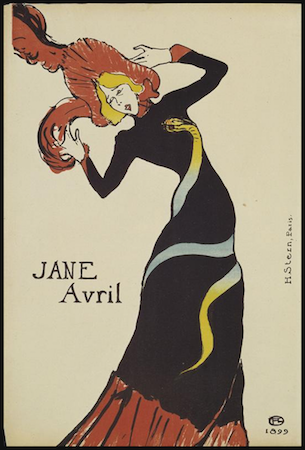
\includegraphics[width=\linewidth]{JaneAvril}
  \caption[Toulouse-Lautrec's `Jane Avril']{Toulouse-Lautrec's `Jane Avril'}
\label{fig:toulouse}
\end{minipage}
\hspace{.05\linewidth}
\begin{minipage}{.45\linewidth}
  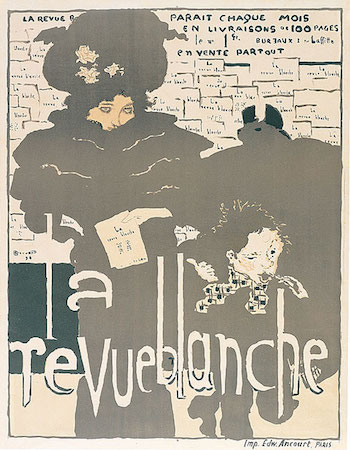
\includegraphics[width=\linewidth]{RevueBlanche}
  \caption[Bonnard's `Revue Blanche']{Bonnard's `Revue Blanche'}
\label{fig:bonnard}
\end{minipage}
\vspace{.05\linewidth}
\begin{minipage}{.45\linewidth}
  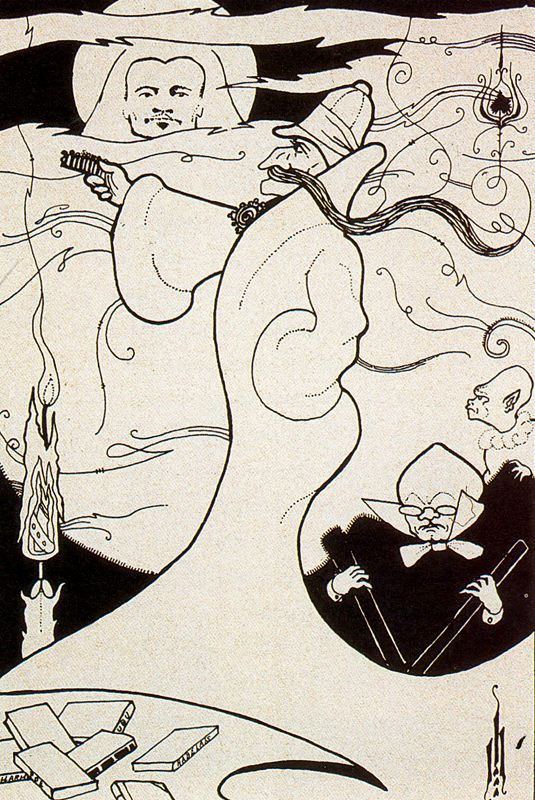
\includegraphics[width=\linewidth]{DocteurFaustroll}
  \caption[Beardsley's `Docteur Faustroll']{Beardsley's `Docteur Faustroll'}
\label{fig:beardsley}
\end{minipage}
\hspace{.05\linewidth}
\begin{minipage}{.45\linewidth}
  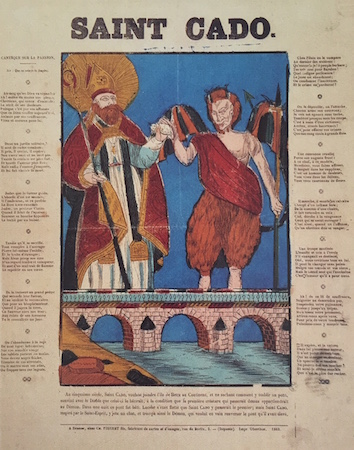
\includegraphics[width=\linewidth]{SaintCado}
  \caption[Oberthuer's `Saint Cado']{Oberthuer's `Saint Cado'}
\label{fig:oberthuer}
\end{minipage}
\end{figure}


\section{100.000.000.000.000 Poems}

The interface design\marginnote{§~\ref{s:poetry}} of some of my search results is directly inspired by
Raymond Queneau's `Cent Mille Milliards de Poèmes', a prime example of Oulipian art \citeyear{Queneau1961}. The book is essentially made up of 10 pages containing one sonnet each. Each page however is split into 14 thin strips, one for each line. This means that mathematically there are $10^{14}$ possible poems to be read by combining different lines every time. My implementation of this resulted in a sonnet, each line of which can be changed individually using mouse clicks.

\begin{figure}[h!]
\centering
\begin{minipage}{.45\linewidth}
  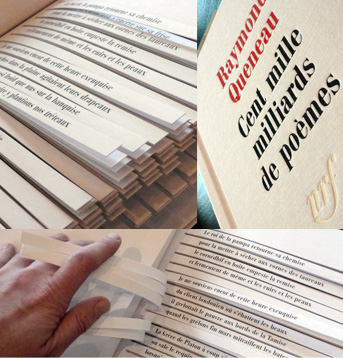
\includegraphics[width=\linewidth]{queneau1}
\end{minipage}
\hspace{.05\linewidth}
\begin{minipage}{.45\linewidth}
  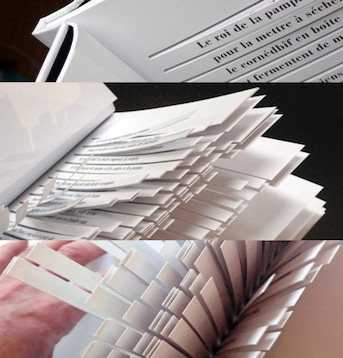
\includegraphics[width=\linewidth]{queneau2}
\end{minipage}
\caption[Queneau's `Cent Mille Milliards de Poèmes']{Raymond Queneau's `Cent Mille Milliards de Poèmes'\footnotemark}
\label{fig:queneau12}
\end{figure}
\footnotetext{Images of Queneau's book in the Gallimard 2006 edition by Martin Pyper \url{http://www.mestudio.info/2010/02/28/one-hundred-thousand-billion-poems/}}
\todo{place footnote text on correct page on final runthrough}


\section{Celestial Emporium of Benevolent Knowledge}

Jorge Luis Borges mentiones a `Chinese Encyclopaedia' called the \emph{Celestial Emporium of Benevolent Knowledge} in the short story `The Analytical Language of John Wilkins' \citeyear{Borges2000}. It is a primary inspiration for this project, originally identified by \autocite{Hendler2011, Hendler2013}. It lists the following results under the category of `animal'.

\begin{quotation}
\begin{enumerate}
  \item those that belong to the Emperor,
  \item embalmed ones,
  \item those that are trained,
  \item suckling pigs,
  \item mermaids,
  \item fabulous ones,
  \item stray dogs,
  \item those included in the present classification,
  \item those that tremble as if they were mad,
  \item innumerable ones,
  \item those drawn with a very fine camelhair brush,
  \item others,
  \item those that have just broken a flower vase,
  \item those that from a long way off look like flies.
\end{enumerate}
\end{quotation}

Although these are obviously all perfectly valid results, it is clear that they form a more creative, even poetic, view of what an animal might be than the Oxford English Dictionary's prosaic: `a living organism which feeds on organic matter' \citeyear{OEDanimal}. This poetic form of order or structure was a direct inspiration for the results generated by this project's exploratory search tool \url{pata.physics.wtf}.


\section{Metaphorical Search Engine Yossarian}

Yossarian is a creative search engine which claims to return `diverse and unexpected results' \citeyear{Yossarian2015}. It is porobably the closest thing to `related work' that exists for this project. Being a commercial product it is hard to find reliable details on precisely how their search engine works. The site seems well marketed but its functionality is shrouded in mystery. However, they argue that

\begin{quotation}
  Yossarian makes the process of generating new ideas faster, while also improving its quality. This creative search engine helps people discover new perspectives, conceptual directions, creative insights, and allowing collaboration and feedback from a creative global community. \sourceatright{\autocite{Yossarian2015}}
\end{quotation}

They also claim to be inspired by metaphors and that generating lateral connections can diversify users ideas and help understand conceptual relationships between things through a `creative graph'.

The site started in a public alpha release in 2012. At the time it consisted of simple image search. In December 2015 a complete re-design was released \autocite{YossarianEmail} which turned the search engine into more of a mind map tool.

\begin{quotation}
  Idea Boards you can now visually jump from idea to idea and build your own custom collection of links. Its a powerful new kind of mind map powered by search, and a radical departure from traditional search engine interfaces. \sourceatright{\autocite{YossarianEmail}}
\end{quotation}

While they do boldly call themselves `the world\rq s first creative search engine' \autocite{Yossarian2015} it is impossible to know how their algorithms really work and as such how similar out projects are. The recently released mind map functionality brings up those `lateral connections' in a relationship graph form, in fact there is a slider that lets users adjust how creative they want their results to be - from literal to lateral.

This search engine appeared some time after I began my PhD research and has been slow to develop. It was hard to find any concrete inspiration from it due to its secrecy and pre-release status. While the marketing and `arty bollocks'\footnote{\url{http://www.artybollocks.com/}} is great, their aim seems to be very different from mine.


\section{The Library of Babel}

The \emph{Library of Babel} is a short story by Jorge Luis Borges \citeyear{Borges1964}. It envisions a universe, called `the Library', which is composed of `an indefinite and perhaps infinite number of hexagonal galleries' containing every possible book every conceived and not yet conceived.

The specific artefact of inspiration for my project is a website implementing a miniature form of this library\footnote{\url{https://libraryofbabel.info/}} created by Jonathan Basile \citeyear{Basile2015}. Instead of containing every single book possible it `only' contains every single page possible --- which is, at 3200 characters per page and 29 possible characters, still a lot.

Basile claims to use a `pseudo-random number generating algorithm' (combining modular arithmetic and bit-shifting operations) to produce all $29^{3200}$ pages without needing to store anything on disk.

\begin{quotation}
  The pages of rational text which this algorithm can locate are rarer than a single grain of sand in that collection, yet intrinsically no more meaningful.
  [\ldots]
  One can find only text one has already written, and any attempt to find it in among other meaningful prose is certain to fail. The tantalizing promise of the universal library is the potential to discover what hasn’t been written, or what once was written and now is lost. But there is still no way for us to find what we don’t know how to look for.
  [\ldots]
  Nonetheless, the library contains its own sort of poetry and revelation, and even this disappointment can provide a moment of clarity. \sourceatright{\autocite{Basile2015}}
\end{quotation}

It is hard to say what exactly influenced my project most. I think the idea of computationally generating this massive library is fantastic --- and absurd. Perhaps this is a feature we share.


\section{The Zen of Python}

The programming language Python was used for the core system behind the \url{pata.physics.wtf} site. The so-called \emph{Zen of Python} is a set of guidelines for good practice in programming originally defined by Guido van Rossum---the creator of Python---who is endeeringly known as the \gls{bdfl} and put into the below form by Tim Peters.

This set of principles is also known as `\acrshort{pep}20'. The abstract reads: `Long time Pythoneer Tim Peters succinctly channels the \acrshort{bdfl}\rq s guiding principles for Python\rq s design into 20 aphorisms, only 19 of which have been written down.' \citeyear{PEP20}

\begin{quotation}
  Beautiful is better than ugly.\\
  Explicit is better than implicit.\\
  Simple is better than complex.\\
  Complex is better than complicated.\\
  Flat is better than nested.\\
  Sparse is better than dense.\\
  Readability counts.\\
  Special cases aren't special enough to break the rules.\\
  Although practicality beats purity.\\
  Errors should never pass silently.\\
  Unless explicitly silenced.\\
  In the face of ambiguity, refuse the temptation to guess.\\
  There should be one-- and preferably only one --obvious way to do it.\\
  Although that way may not be obvious at first unless you're Dutch.\\
  Now is better than never.\\
  Although never is often better than *right* now.\\
  If the implementation is hard to explain, it's a bad idea.\\
  If the implementation is easy to explain, it may be a good idea.\\
  Namespaces are one honking great idea -- let's do more of those!
  \sourceatright{\autocite{PEP20}}
\end{quotation}

I cannot claim to have followed each and every one of those recommendations in my coding practice (although I have certainly tried) but it has been highly influential during the writing and design of this thesis.

\spirals

The following list shows some other general programming culture references that have been inspirational in one way or another. They were interesting to me due to their underlying sense of humour which resembles that of pataphysics.

\begin{description}
  \item [Jargon File] a `comprehensive compendium of hacker slang illuminating many aspects of hackish tradition, folklore, and humor'\footnote{See \url{http://www.catb.org/~esr/jargon/}}
  \item [Code Golf] `a competition to solve a particular problem in the fewest bytes of source code'\footnote{See \url{http://codegolf.stackexchange.com/questions/tagged/code-golf}}
  \item [Code Bowling] `a competition to solve a particular (usually simple) problem in the most bytes or complexity'\footnote{See \url{http://codegolf.stackexchange.com/questions/tagged/code-bowling}}
  \item [\gls{ioccc}] a competition to `write the most obscure/obfuscated C program within the rules to show the importance of programming style, in an ironic way'\footnote{See \url{http://www.ioccc.org/}}
  \item [Glitch Art] Wikipedia defines it as `the aestheticization of digital or analog errors, such as artifacts and other `bugs', by either corrupting digital code/data or by physically manipulating electronic devices (for example by circuit bending)'\footnote{See \url{https://www.reddit.com/r/glitch_art/} and \url{https://goo.gl/waiqKV}}
  \item [Easter Eggs] The practice of hiding a reproducible, personal, harmless and entertaining feature into a piece of software \footnote{See \url{http://www.eeggs.com/faq.html}}
  \item [Knuth] \footnote{See \url{http://www-cs-faculty.stanford.edu/~uno/help.html}}
\end{description}

\todo{finish writing these out}


\stopcontents[chapters]
